%% ############################################################################
%% Unterkapitel
%% ############################################################################
\section{ Web-Programmierschnittstelle (Web-API)}
Für die neue Webseite und für andere Anwender ist eine API (application programming interface) erstellt worden. Um eine API zu entwickeln muss zuerst verstanden werden was eine API ist. Deswegen werden zu beginn folgende Fragen gestellt und beantwortet.
\begin{itemize}
\item Was ist eine API?
\item Wie wird eine API entwickelt?
\item Was ist state of the Art?
\end{itemize}

Anschliessend wird in diesem Kapitel aufgezeigt wie die API entwickelt wurde und wo diese zum Einsatz kommt.

\subsection{Was ist eine API?}
Eine API überbrückt die Schnittstellen zwischen verschiedenen Software teilen und strukturiert die dabei anfallende Datenübergabe dazwischen. Sie ermöglicht es Software zu modularisieren und die Kommunikation zu vereinfachen. Konkret heisst dies, dass die einzelnen Programmteile  voneinander ab gekapselt werden und kommunizieren nur über die Festgelegte API. Der Vorteil hierbei ist, das die API veröffentlicht werden kann und somit auch anderen die Möglichkeit gegeben werden kann die angebotenen Dienste mittels der API zu erhalten. Zusätzlich können so auch die einzelnen modularisierte Softwareteile unabhängig voneinander weiterentwickelt werden. Nicht zuletzt ist auch das Testen ein wichtiger Punkt, da alle Programmteile nur über die API miteinander kommunizieren sollten muss die Software auch nur in der Zusammenarbeit mit der API getestet werden.

\subsection{Was ist state of the Art?}
Heutzutage wird werden viele API nach dem RESTful Standard entwickelt wird. Da taucht die Frage auf was ist RESTful? Ein kleiner Exkurs. RESt steht für State Transfer und ist im Gegensatz zu Protokollen eine Philosophie, welche die Möglichkeiten von HTTPS ausnutzt. REST benötigt hierfür die von HTTPS bekannten CRUD Verben (Create, Read, Update, Delete) \cite{LornaJaneMitchell2013oreilly}. Im Vordergrund bei REST steht die Zustandslosigkeit, das heisst Server sowie Client haben keinen Zustand zwischen den Anfragen. Eine Verbindung bleibt jedoch bis zum Ende der Anwendung oder Nutzzeit bestehen. Ein Beispiel für diese Zustandslosigkeit ist in Abb. \ref{img:Sequenzdiagramm_API} zu sehen.\\

\begin{figure}[h!]
	\centering
	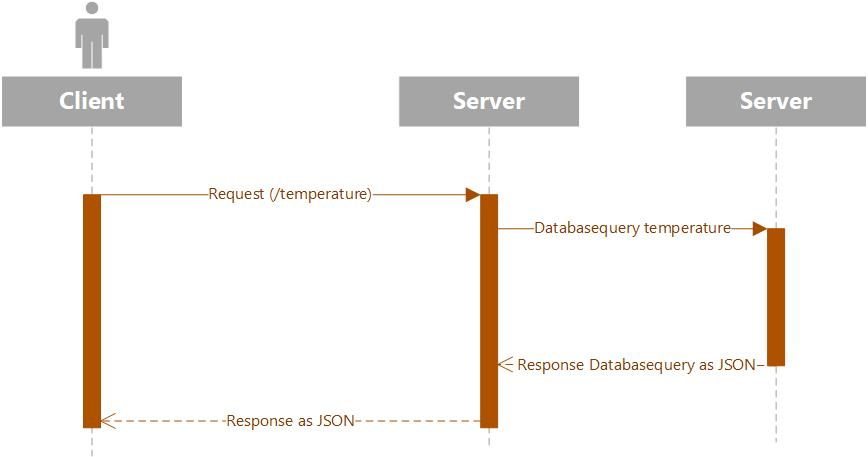
\includegraphics[width=1\linewidth]{img/Sequenzdiagramm_API}
	\caption{Beispiel einer API GET-Abfrage}
	\label{img:Sequenzdiagramm_API}
\end{figure}


\subsection{Wie wird eine API entwickelt?}
Zu Beginn der Entwicklung muss klar sein für was die API benötigt wird. Ist dies klar, kann gesagt werden welche Anforderungen die API erfüllen muss. Als nächstes muss ein URL Schema her. Dies wird benötigt um nach dem REST Standard zu arbeiten. Die URL sollte folgendermassen aussehen: \\ https://api.wetter-arbon.ch/Versionsnummer/Endpunkt\\
Die Versionsnummer wird zur Weiterentwicklung benötigt. Wird beispielsweise eine neue Version der API veröffentlicht, kann es sein das nicht alle Nutzer der API auf die neue Version umgestiegen sind. Somit kann es geschehen, dass die vorhandenen Installationen zerstört werden. Neben der URL ist es wichtig das die Kommunikation in einem bestimmten Datenformat erfolgt, hier gibt es die Möglichkeit zu wählen zwischen JSON, XML oder CSV. Es können auch andere Formate genutzt werden. Wichtig ist jedoch, dass der Server sowie der Client wissen welches. Nebst der Entwicklung für die Server-Client Kommunikation ist auch bei der API eine Zugangskontrolle bzw. eine Grundbasis in der Sicherheit notwendig. Neben der Möglichkeit HTTPS zu verwenden, ist es zusätzlich möglich den Client über einen sogenannten Authorization Token zu zu authentifizieren. Eine andere Möglichkeit ist, den Zugriff durch eine IP-Whitelist zu begrenzen. \\


\subsection{API Konzept}
Nachdem die Fragen zur API beantwortet sind kann die API für die Wetterstation Arbon Konzipiert und umgesetzt werden. Für die API gibt es jedoch eine wichtige Bedingung. Sie muss in php geschrieben werden, da Hostpoint kein Javascript auf der Serverseite erlaubt.

Zu Beginn des API Konzept sollten die Anforderungen daran erstellt werden. Die API soll mindestens folgende Datenpunkte enthalten:
\begin{itemize}
\item Wind / Windrichtung
\item Niederschlag
\item Temperatur / Gefühlte Temperatur
\item Luftfeuchtigkeit
\item Wassertemperatur (1m Unter der Wasseroberfläche)
\item Wassertemperatur (Oberfläche)
\item Wasserpegel
\item Wellenhöhe
\item Radiation /daily sunduration
\item Webcam
\item Sturmwarnung
\end{itemize}
Die Datenabfrage über die API soll wie es State of the Art entwickelt wird RESTful sein und mittels HTTP geschehen. Mit der API werden nur GET-Anfragen erlaubt sein, da bspw. keine POST-Befehle oder sonstige Befehle ausgeführt werden müssen. Somit ist ein sogenannter Token für die Authentifizierung nicht notwendig. Das Datenformat der API soll JSON sein. JSON ist ein simples Datenformat, welches nicht viel Speicherplatz benötigt und somit auch einfach Transferiert werden kann. Nebst der Lesbarkeit für Menschen, kann es auch von Maschinen gelesen werden. Javascript beispielsweise handhabt JSON nativ. Nebst dem das Javascript JSON versteht, ist auch die Handhabung bei PHP simpel  \Diskussionspunkt{LITERATUR}. 

\paragraph{JSON Struktur}

Um die API zu entwickeln wurden die Anforderungen in einen sogenannten JSON-tree (siehe \Diskussionspunkt{ANHANG}) umgeformt. Hieraus wird auch die URL entstehen zur Abfrage der Daten. Der Aufruf wird Grundsätzlich über api.wetter-arbon.ch gemacht um einzelne Werte abzufragen muss tiefer in die Verzeichnisse gegangen werden.


\subsection{Umsetzung der API}
Jetzt wo die Struktur steht kann auch das Konzept umgesetzt werden. Das Verzeichnis soll gemäss Abb. \ref{img:APIVerzeichnis}aufgebaut werden.


\begin{figure}[h!]
	\centering
	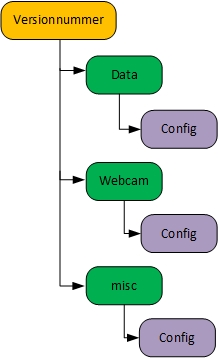
\includegraphics[width=0.3\linewidth]{img/APIVerzeichnis.jpg}
	\caption{Aufbau des API Verzeichnis}
	\label{img:APIVerzeichnis}
\end{figure}

Für diesen Aufbau wurde gewählt, weil so die API erweiterbar bleibt und klar strukturiert ist. Im Verzeichnis Data werden die alle Sensordaten verarbeitet, im Verzeichnis Webcam wird nur das JSON für die Webcam erstellt, da hier keine Datenbankabfrage notwendig ist und im Verzeichnis misc werden verschiedene Daten von dritten verarbeitet.

\paragraph{PHP Files}
In diesem Unterkapitel geht es um den Grundaufbau der verschiedenen PHP Files welche im Verzeichnis Data und misc benötigt werden, zudem wird aufgezeigt wie weitere Sensordaten hinzugefügt werden können um die Modularität aufzuzeigen. Vom Grundaufbau sind die Dateien im Config-Ordner und der Ablauf der Anfragen wie in Bild \ref{img:APIFiles}
\begin{figure}[h!]
	\centering
	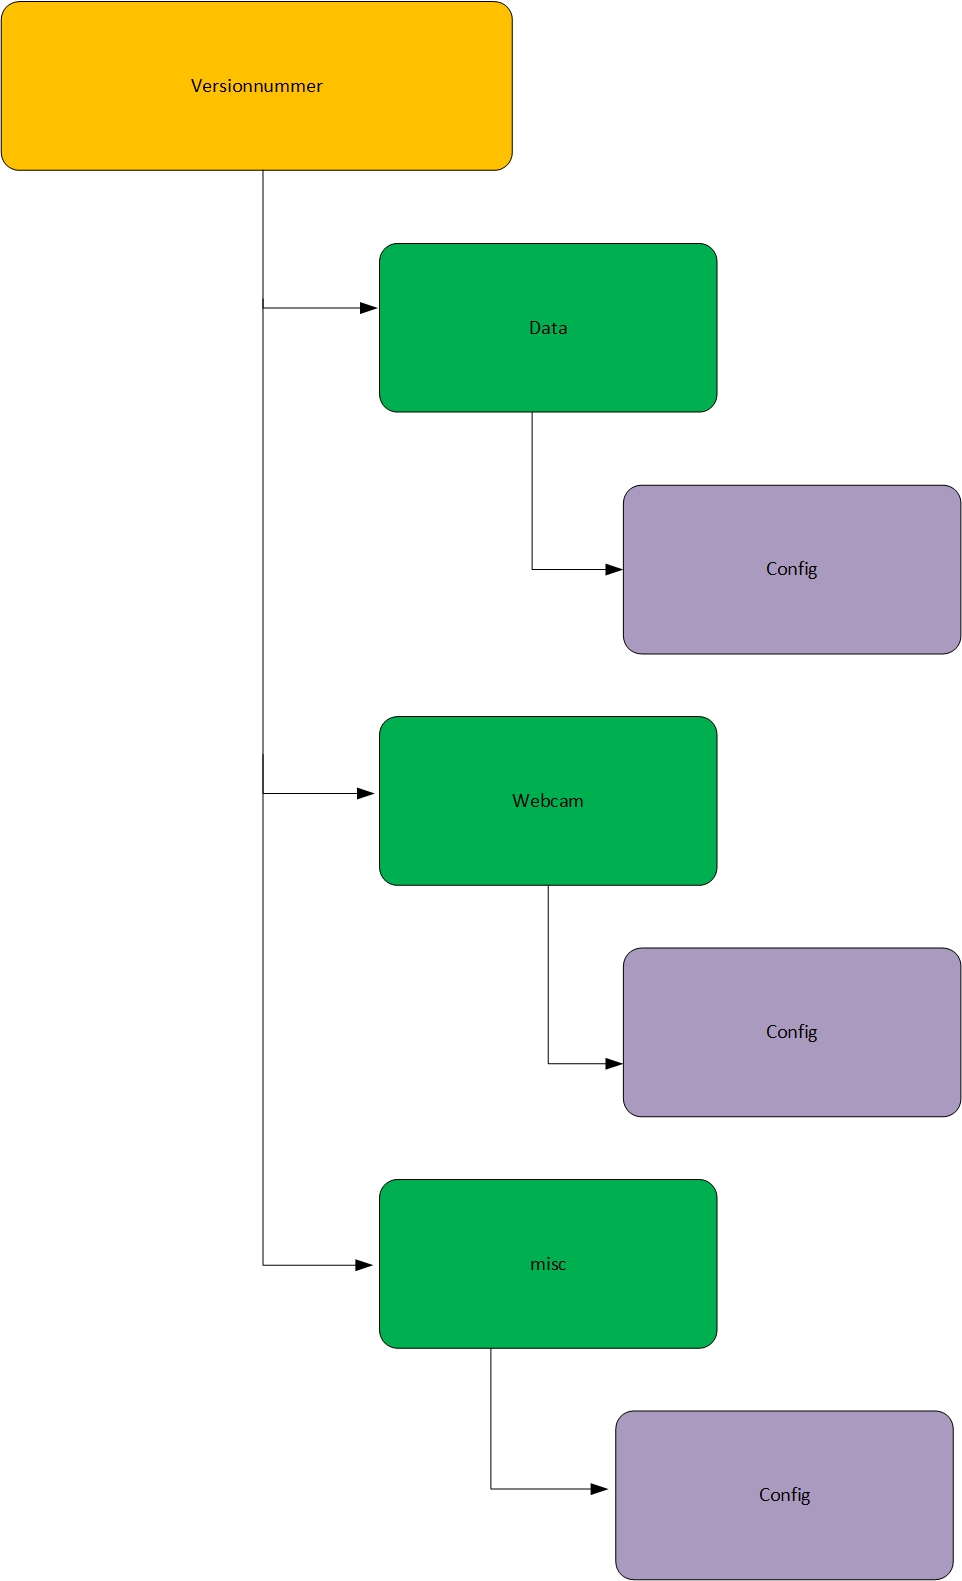
\includegraphics[width=0.5\linewidth]{img/APIFiles.jpg}
	\caption{PHP Files und Ablauf einer Abfrage}
	\label{img:APIFiles}
\end{figure}


Im File Path \ref{lst:path} wird die URL ausgelesen und dem richtigen Case zugewiesen. Siehe Bild. In der Zeile 2 wird die URL für den case überprüft. Ist diese richtig, wird der entsprechende Tabellenname in der dieses Attribut vorhanden ist angegeben, dies ist für die Datenbankabfrage. Anschliessend wird angegeben welche Sensorwerte aus der Datenbank benötigt werden. In Zeile 12 wird das sogenannte dataJsonStatic erstellt, hierbei wird die Beschreibung (description) und die Einheit (unit) der Daten angegeben. Grund für diesen Arraynamen ist das diese Daten statisch sind. Anschliessend wird der JSON Name vergeben in Zeile 17. Zum Schluss in Zeile 20 wird die entsprechende Funktion im createJson aufgerufen mit der entsprechenden Parameterliste

\begin{lstlisting}[label=lst:path,caption=Beispiel Case zuweisung, language=php, style=php]
  //if the case is the right URI do case
    case "/v1/data/temperature": //temperature
      //set table name for SQL query
      $table = "tblwettertransmitter";
      //set required parameters for SQL query
      $requiredData=array(
        "value" => "temperature",
        "min"  => "min_daily_temperature",
        "max" => "max_daily_temperature"
      );
      //set the static Json data
      $dataJsonStatic=array(
        "description"  => "Lufttemperatur",
        "unit"  => "C"
      );
      //Set the Json Name
      $name = "temperature";
    //call function createJson to do the SQL query and make a Json. Function is in file createJson.php

      createJsonMinMax($requiredData, $dataJsonStatic, $table, $name);
    break;
\end{lstlisting}

Nachdem die Funktion aufgerufen worden ist, geht es ins File createJson. Im File createJson bestehen verschiedene Funktionen, passend zur Anforderung. Es bestehen folgenden Funktionen welche kurz umschrieben werden welches Ziel diese haben.\\
\begin{itemize}
\item CreateJsonMinMax
\begin{itemize}
\item Diese Funktion erstellt die JSONs mit dem aktuellen Wert sowie den Extrema des Tages
\end{itemize}
\item CreateJson
\begin{itemize}
\item Erstellt das Json für die Daten, welche keine Extrema oder sonstige umrechnungen benötigen
\end{itemize}
\item CreateJsonConversion
\begin{itemize}
\item Erstellt das Json für die Windgeschwindigkeiten mit den verschiedenen Einheiten Km/h, knoten und beufort. Umgerechnet werden die aktuellen Werte, sowie die Extrema
\end{itemize}
\item createJsonSunduration
\begin{itemize}
\item Rechnet die Sonnenminuten des Tages in Stunden um und erstellt das entsprechende Json Format
\end{itemize}
\end{itemize}

Zurück zum Beispiel für den Aufruf des Temperatur Jsons. In der Zeile 4 und 5 wird die Verbindung zur Datenbank hergestellt \ref{lst:createJson}, dazu später mehr. Anschliessen wird die Klasse Sensors initialisiert und der Variable data zugewiesen und in der Zeile 8 die Datenbankabfrage durchgeführt und das Resultat in der Variablen stmt gespeichert. Nachdem die Datenbankabfrage erfolgreich wird das Resultat mittels einer while-Schlaufe in die einzelnen Spalten zerlegt und als Array gespeichert. Von Zeile 14 bis 22 wird das assoziative Array dataJson aufgebaut um in der Zeile 24 mit dem Array im File path.php zusammengefügt zu werden. Anschliessen wird das Array mittel einem echo zurückgegeben. Die restlichen Funktionen unterscheiden sich nur im Aufbau des Arrays, die Datenbankabfrage, das Aufbauen des dataJson und das Zusammenfügen sowie das zurückgeben funktioniert überall gleich.

\begin{lstlisting}[label=lst:createJson,caption=Beispiel erstellung des Jsons, language=php, style=php]
function createJsonMinMax($requiredData, $dataJsonStatic, $table,$name)
{
  // instantiate database and data object
  $database = new Database();
  $db = $database->getConnection();
  $data = new Sensors($db);
  //call function readMinMax to get the database data
  $stmt = $data->readMinMax($requiredData, $table);

  while ($row = $stmt->fetch(PDO::FETCH_BOTH))
  {
    extract($row);
    //create Json from DB results
    $dataJson=array(
      "value" => (float)$row[1],
      "dailymax" => (float)$row[3],
      "dailymin" => (float)$row[2],
      "timestamp" => $row[0],
      "interval"  => 60,
      "intervalUnit" => "seconds"
    );
  }
  //merge static data array and DB array
  $jsonArray[$name]=array_merge_recursive($dataJsonStatic, $dataJson);
  //encode to Json
  echo json_encode($jsonArray);
}



\end{lstlisting}
Vor das die Datenbankabfrage \ref{lst:database} ausgeführt werden kann, muss eine Datenbankverbindung hergestellt werden. Hier wird Gebrauch vom try, catch Verfahren gemacht. Hiermit ist es möglich wie auch in anderen Programmiersprachen eine Ausnahme (Exception) abgefangen werden \cite{Ausnahmebehandlung:ThePHPGroup}. In der Zeile 7 d.h. im try wird die Verbindung durch eine Instanz der PDO Klasse erzeugt. Diese benötigt die richtigen Parameter für die Verbidung, d.h. den host, den Datenbanknamen, den Datenbankbenutzer und das Passwort.

\begin{lstlisting}[label=lst:database,caption=Beispiel Aufbau der Datenbankverbindung, language=php, style=php]

  // get the database connection
  public function getConnection()
  {
    $this->conn = null;

    try
    {
      $this->conn = new PDO("mysql:host=" . $this->host . ";dbname=" . $this->db_name, $this->username, $this->password);
      $this->conn->exec("set names utf8");
    }
    catch(PDOException $exception)
    {
      echo "Connection error: " . $exception->getMessage();
    }

    return $this->conn;
  }


\end{lstlisting}
Nachdem die Verbindung aufgebaut ist, wird wie bei der erklärung für das CreateJson und deren Funktion erwähnt die Datenbankabfrage durchgeführt. In Zeile 16 wird die Abrage erstellt, im Beispiel für die Temperatur würde für die variablen folgende Strings stehen:\\
\begin{lstlisting}[label=lst:createJson,caption=Beispiel erstellung des Jsons, language=php, style=php]
$requiredData['value'] -> temperature
$requiredData['min'] -> min_daily_temperature
$requiredData['max'] -> max_daily_temperature
$table ->  tblwettertransmitter
\end{lstlisting}
Diese Werte würden vorher aus der Funktion creatJsonMinMax übergeben. Ist die Query erstellt, wird diese in Zeile 3 vorbereitet und in Zeile 14 ausgeführt. Nachdem diese Ausgeführt wurde wird sie zurückgegeben an die Funktion createJsonMinMax wo die Resultate wie beschrieben aufbereitet werden zu einem Json.

\begin{lstlisting}[label=lst:createJson,caption=Beispiel erstellung des Jsons, language=php, style=php]
function readMinMax($requiredData, $table)
  {
    $query= "SELECT datetime,".$requiredData['value'].", ".$requiredData['min'].", ".$requiredData['max']."
    FROM ".$table." WHERE datetime = (SELECT MAX(datetime) FROM ".$table.");";

    // prepare query statement
    $stmt = $this->conn->prepare($query);
    /*
    $stmt->bindParam(':valuename', $requiredData['value']);
    $stmt->bindParam(':minname', $requiredData['min']);
    $stmt->bindParam(':maxname', $requiredData['max']);
*/
    // execute query
    $stmt->execute();

    return $stmt;
  }



\end{lstlisting}
